% !Mode:: "TeX:UTF-8"
% !TEX program  = xelatex
\documentclass[a4paper]{article}
\usepackage{amsmath}
\usepackage{amssymb}
\usepackage[page]{appendix}
\usepackage{bm}
\usepackage{ctex}
\usepackage{caption}
%\usepackage{braket}
%\usepackage[european]{circuitikz}
\usepackage{multirow}
\usepackage{float}
\usepackage{graphicx}
\usepackage{geometry}
\geometry{left=2.5cm,right=2.5cm,bottom=2.5cm,top=2.5cm}
\title{近代物理实验报告9.3:光磁共振}
\author{xy\quad 学号\quad 匡亚明学院}
\date{2019年2月29日}
\begin{document}
\maketitle
\bibliographystyle{unsrt}
%--------main-body------------

\section{引言}
为了研究物质内部不同层次的结构和性质,利用电磁波与物质的相互作用作为研究手段,最早使用的是光谱学方法,取得有关原子、分子结构的大量数据,促进了原子、分子物理学的发展,但由于仪器分辨率和谱线线宽的限制,对原子、分子等微观粒子内部更加精细的结构和性质得不到满意的结果,后来发展了波谱学的方法,直接观测在外磁场中原子精细结构能级、超精细结构能级和塞曼子能级间的微波或射频共振(通常称为磁共振)。分辨率提高了,但是跟微波或射频共振相联系的能级间的能量差很小,由玻尔兹曼分布所造成的粒子在能级上的分布的布居数之差也很小,而且磁偶极跃迁几率比电偶极跃迁几率小几个数量级,磁共振信号很弱,难于探测,迫切需要提高共振信号的强度。凝聚态物质的波谱学如核磁共振、电子顺磁共振,实验样品浓度较大,加上高灵敏度的电子技术探测方法,可以获得很好的共振信号,在很多领域得到应用。然而对于研究自由原子的气态波谱学来说,由于样品浓度低几个数量级,共振信号极弱,必须设法提高共振信号强度,才能进行实验观测。为此,法国物理学家卡斯特勒(A. Kastler)在20世纪50年代提出光磁共振技术,即光泵磁共振或光抽运磁共振技术。这是让原子、分子等样品在弱磁场(约$10^{-5}\sim 10^{-4}$T)、光频和射频地磁场的共同作用下,使光频电共振跃迁和射频磁共振跃迁共同发生的一种双共振技术。气体原子样品置于弱磁场和射频磁场中,在弱磁场的作用下其超精细结构能级分裂成塞曼子能级,用圆偏振$\sigma^{+}$光(或$\sigma^{-}$光)入射到气态原子样品上,原子吸收入射光产生光抽运(Optical Pumping),使绝大多数原子处于基态的最高的(或最低的)塞曼子能级上。同时在射频磁场的作用下产生射频磁共振,测量通过样品的透射光,能获得发生射频磁共振的信号。由于光抽运造成相邻塞曼子能级上粒子数的差额比玻尔兹曼分布造成的粒子数差额要大几个数量级,而且光频信号(光子能量$10^{-1}\sim 1$eV)比射频信号(光子能量约$10^{-8}$eV)的能量大大提高,因此这种光磁共振技术使得对射频磁共振的探测变得容易起来,它既保持了磁共振的高分辨率,又比直接探测射频磁共振信号将探测灵敏度提高了七八个甚至十几个数量级,因而特别适用于研究原子、分子能级的精细结构、超精细结构的其它各种参量的精密测量,以及对原子、分子间相互作用和它们与其他物质的相互作用进行实验研究。典型的光磁共振方法是按照“光抽运-磁共振-光探测”的思想来研究原子精细结构的一种实验方法。利用光磁共振原理以及开发出两类精密仪器:原子时间频率标准(原子钟)和原子磁强计,它们广泛应用于科学技术的各个领域中。20世纪80年代初出现的激光-射频双共振技术在原子、分子高激发态的精密测量方面也获得广泛的应用。卡斯特勒由于在发现和发展研究原子的光磁双共振方法中作出的贡献,获得1966年诺贝尔物理学奖。

\section{实验目的}
\begin{enumerate}
\item 掌握“光抽运-磁共振-光探测”的思想方法和实验技巧,研究原子超精细结构塞曼子能级间的射频磁共振。
\item 测定銣原子$^{87}$Rb和$^{85}$Rb的参数:基态朗德因子$g_F$和原子核的自旋量子数$I$。
\item 测定地磁场$\bm{B}_\text{地}$的垂直分量$B_{\text{地垂直}}$、水平分量$B_{\text{地水平}}$及其倾角$\theta$。
\end{enumerate}

\section{实验仪器}
光(泵)磁共振实验仪、射频信号发生器、数字频率计、二通道型数字存储示波器、直流数字电压表等。

\section{实验原理}
光磁共振技术是根据动量守恒原理,用光学抽运来研究原子超精细结构塞曼子能级间微波或射频磁共振现象的双共振技术。特点是兼有波谱学方法的高分辨率和光谱学方法的高探测灵敏度。
\subsection{铷原子的超精细结构及其塞曼分裂}
铷是一价碱金属原子,有一个价电子,处于第五壳层,主量子数$n=5$,电子轨道量子数$L=0$, $1$, $\dots$, $n-1=4$,电子自旋$S$=$\frac{1}{2}$。铷原子中价电子的轨道角动量$\bm{P}_L$和自旋角动量$\bm{P}_S$发生轨道-自旋耦合($LS$耦合),得到电子总角动量$\bm{P}_J$,其数值$P_J = \sqrt{J(J+1)}\hbar$,$J=L+S$, $L+S-1$, $\dots$, $|L-S|$。当不考虑铷原子核的自旋时,铷原子总磁矩$\mu_J = -g_J\frac{e}{2m_e}P_J$,其中$-$e,$m_e$分别为电子的电荷、质量。朗德因子
\begin{equation}
g_J = 1+\frac{J(J+1)- L(L+1)+ S(S+1)}{2J(J+1)}\label{eq1}
\end{equation}
从而形成原子的超精细结构能级,这时,铷原子的基态能级$n^{2S+1}\text{S}_J$对应于$n=5$,$L=0$,$S=\frac{1}{2}$,$J=\frac{1}{2}$,即为$5^2\text{S}_{\frac{1}{2}}$,相应的朗德因子$g_J$=2;铷原子的第一激发态能级$n^{2S+1}\text{P}_J$对应于$n=5$,$L=1$,$S=\frac{1}{2}$,$J=\frac{1}{2}$、$\frac{3}{2}$,是双重态,即为$5^2\text{P}_{\frac{1}{2}}$和$5^2\text{P}_{\frac{3}{2}}$,相应的朗德因子$g_J=\frac{2}{3}$,$\frac{4}{3}$。$5^2\text{P}_{\frac{1}{2}}\to 5^2\text{S}_{\frac{1}{2}}$的能级跃迁产生光谱线$D_1$线($\lambda_1=794.76$nm);$5^2\text{P}_{\frac{3}{2}}\to 5^2\text{S}_{\frac{1}{2}}$的跃迁产生光谱线$D_2$线($\lambda_2=780.0$nm)。本实验观测与$D_1$线有关的能级的超精细结构及其在弱磁场中的塞曼分裂。

通常原子核也具有角动量,记原子核的总角动量为$\bm{P}_I$,它是核中质子和中子的轨道角动量和自旋角动量的矢量和,核的总角动量的数值$P_I=\sqrt{I(I+1)}\hbar$,通常也称为核自旋,其中I称为核的自旋量子数,$I$为整数或半整数,已知稳定的原子核的$I$值在0到$\frac{15}{2}$之间。核的总角动量$\text{P}_I$的最大可测的分量值为$I\hbar$。当$I\neq 0$时,原子核的总磁矩为
\begin{equation*}
\mu_I = g_I\frac{e}{2m_p}P_I = g_I\sqrt{I(I+1)}\mu_N
\end{equation*}
朗德因子$g_I$的具体数值还没法由其它量子数算出来,只能由实验测定。$\mu_N = \frac{e\hbar}{2m_p}$称为核磁子,质子质量$m_p$是电子质量$m_e$的1836倍,因此核磁子$\mu_N$比玻尔磁子$\mu_B = \frac{e\hbar}{2m_e}$小三个数量级。原子核总角动量$\bm{P}_I$和电子总角动量$\bm{P}_J$耦合(称为$IJ$耦合)成原子总角动量$\bm{P}_F$,其数值$P_F = \sqrt{F(F+1)}$,$F$为原子总角动量量子数:$F=I+J$, $I+J-1$, $\dots$, $|I-J|$。$F$不同取值的个数为$2I+1$(当$I\leq J$)或$2J+1$(当$J\leq I$)。从而原子的精细结构能级细分为由总量子数$F$标定的超精细结构能级。天然铷中主要含有两种同位素:$^{87}$Rb和$^{85}$Rb,其含量分别约为28\%和78\%。提纯后的$^{87}$Rb和$^{85}$Rb非常昂贵,本实验使用天然铷,既可以同时观测两种铷原子的光磁共振现象,又大大降低实验器材费用。原子的基态$5^2\text{S}_{\frac{1}{2}}$和第一激发态$5^2\text{P}_{\frac{1}{2}}$都分成两个超精细结构能级,对$^{87}$Rb而言,$I=\frac{3}{2}$,分别由量子数$F=I+J=2$和$F=I-J=1$来表征;而对$^{85}$Rb,$I=\frac{5}{2}$,则由$F=3$和$F=2$来表征。原子总角动量$\bm{P}_F$与原子总磁矩$\bm{\mu}_F$之间的关系为:
\begin{eqnarray}
\bm{\mu}_F &=& -g_F\frac{e}{2m_e}\bm{P}_F\label{eq2}\\
g_F &=& g_J\frac{F(F+1) + J(J+1) - I(I+1)}{2F(F+1)}\label{eq3}
\end{eqnarray}
导出上面两个式子时本应包含两项,分别与$\mu_I$和$\mu_J$有关,由于跟$\mu_I$有关的项比跟$\mu_J$有关的另一项要小得多,因此被略去了。

在弱的外磁场中,由于磁场较弱未能破坏$IJ$耦合,必须考虑原子核的总角动量和原子核的总磁矩的影响,用$IJ$耦合后的$\bm{P}_F$和$\mu_F$作为原子的总角动量和总磁矩。本实验中作为非磁性物质的铷原子处于弱磁场$\bm{B}$(通常表征磁场的物理量,在非磁性物质中和磁性物质的外部用磁感应强度$\bm{B}$,在磁性物质内部用磁场强度$\bm{H}$)中,铷原子获得附加的能量$E_{m_F} = -\bm{\mu}_F\bm{\cdot}\bm{B} = m_Fg_F\mu_BB$,其中$\mu_B$为玻尔磁子,磁量子数$m_F=F$, $F-1$, $\dots$, $-F$,共$2F+1$个数值,因此对应于总量子数F的超精细结构能级分裂成$2F+1$个塞曼子能级。相邻子能级之间的数量差均为$E_{m_F} - E_{m_F-1} = \Delta E = g_F\mu_BB$。当外磁场$B=0$时,塞曼子能级简并为超精细结构能级。

铷原子$^{87}$Rb和$^{85}$Rb的基态$5^2\text{S}_{\frac{1}{2}}$和第一激发态$5^2\text{P}_{\frac{1}{2}}$的朗德因子$g_F$和相邻塞曼子能级间能量间隔$|\Delta E| = |g_F|\mu_B|B|$的理论值列在表(\ref{table1})中。
\begin{table}[!h]
\centering
\caption{$g_F$和相邻塞曼子能级间能量间隔$|\Delta E|的理论值$}\label{table1}
\begin{tabular}{|c|c|c|c|c|c|c|}
\hline
$^{87}$Rb                                    & F & J                          & I                          & $g_J$                       & $g_F$理论值   & $|\Delta E|$理论值                    \\ \hline
\multirow{2}{*}{$5^2\text{P}_{\frac{1}{2}}$} & 2 & \multirow{2}{*}{$\frac12$} & \multirow{2}{*}{$\frac32$} & \multirow{2}{*}{$\frac23$} & $\frac16$  & \multirow{2}{*}{$\frac16\mu_B|B|$} \\ \cline{2-2} \cline{6-6}
                                             & 1 &                            &                            &                             & $-\frac16$ &                                    \\ \hline
\multirow{2}{*}{$5^2\text{S}_{\frac{1}{2}}$} & 2 & \multirow{2}{*}{$\frac12$} & \multirow{2}{*}{$\frac32$} & \multirow{2}{*}{2}          & $\frac12$  & \multirow{2}{*}{$\frac12\mu_B|B|$} \\ \cline{2-2} \cline{6-6}
                                             & 1 &                            &                            &                             & $-\frac12$ &                                    \\ \hline
\end{tabular}

\begin{tabular}{|c|c|c|c|c|c|c|}
\hline
$^{85}$Rb                                    & F & J                          & I                          & $g_J$                      & $g_F$理论值   & $|\Delta E|$理论值                    \\ \hline
\multirow{2}{*}{$5^2\text{P}_{\frac{1}{2}}$} & 3 & \multirow{2}{*}{$\frac12$} & \multirow{2}{*}{$\frac52$} & \multirow{2}{*}{$\frac23$} & $\frac19$  & \multirow{2}{*}{$\frac19\mu_B|B|$} \\ \cline{2-2} \cline{6-6}
                                             & 2 &                            &                            &                            & $-\frac19$ &                                    \\ \hline
\multirow{2}{*}{$5^2\text{S}_{\frac{1}{2}}$} & 3 & \multirow{2}{*}{$\frac12$} & \multirow{2}{*}{$\frac52$} & \multirow{2}{*}{2}         & $\frac13$  & \multirow{2}{*}{$\frac13\mu_B|B|$} \\ \cline{2-2} \cline{6-6}
                                             & 2 &                            &                            &                            & $-\frac13$ &                                    \\ \hline
\end{tabular}
\end{table}

在热动平衡条件下,原子在各能级的分布数遵循玻尔兹曼分布($N = N_0e^{-\frac{E}{k_BT}}$),由于基态各塞曼子能级的能量差很小,故可认为原子均衡地分布在基态各塞曼子能级上。如果在引起超精细结构能级分裂的弱磁场的垂直方向上加一个射频磁场,当射频光子能量等于基态相邻塞曼子能级的能量间隔$|\Delta E|$时,$h\nu = |g_F|\mu_B|B|$,会诱导产生这些子能级间的磁共振跃迁,当一个原子发射一份射频光子能量,向下跃迁到相邻塞曼子能级上,但是宏观上没有电磁能量的净吸收或净发射,因而无法从实验上检测出这种磁共振跃迁。若要从实验上检测出磁共振跃迁必须在基态塞曼子能级之间造成显著的粒子数差。光抽运现象就起到这样的作用。
\subsection{圆偏光对铷原子的光抽运效应}
以铷光谱灯发射的$D_1$光入射到铷蒸气原子样品上时,会产生原子在基态$5^2\text{S}_{\frac{1}{2}}$的塞曼子能级与第一激发态$5^2\text{P}_{\frac{1}{2}}$的塞曼子能级之间的跃迁,这种光跃迁起作用的是光的电场部分,必须满足能量守恒和角动量守恒,其选择定则为$\Delta L = \pm 1$,$\Delta F = 0\text{, }\pm 1$,$\Delta m_F = 0\text{, }\pm 1$。如果用的是$D_1\sigma^{+}$光,它是电场矢量绕磁场方向左旋的圆偏光,在磁场方向,角动量为$+\hbar$,它与原子相互作用时,原子不仅吸收光子的能量,也吸收光子的角动量。原子的角动量增加了$+\hbar$值,因而只能发生 $\Delta m_F = +1$的跃迁。由于$^{87}$Rb的基态$5^2\text{S}_{\frac{1}{2}}$和第一激发态$5^2\text{P}_{\frac{1}{2}}$的$m_F$最大值都是$+2$,基态$5^2\text{S}_{\frac{1}{2}}$中$m_F\neq +2$的塞曼子能级上的原子跃迁到激发态$P_I$的允许子能级上,而处于基态的$m_F= +2$子能级上的原子不能跃迁,否则违反了选择定则。原子从$P_I$态会发射光子自发退激返回基态,这是无辐射跃迁,按选择定则$\Delta m_F = 0\text{, }\pm 1$,以同样的概率返回基态各子能量,从而使得基态的 子能级上的原子数增加。经过若干次激发和退激后,基态的$m_F = +2$子能级上的原子数大大增加,好像基态的$m_F\neq +2$的较低子能级上的大量原子被“抽运”到基态基态的$m_F = +2$的子能级上,造成粒子数反转,这就是光抽运效应(亦称“光泵”)。光抽运造成原子的非平衡分布,随着基态的$m_F\neq +2$子能级上原子数的减少,$^{87}$Rb原子对光的吸收减弱,直至饱和不再吸收。$m_F$的每一个数值代表原子总磁矩$\mu_F$在磁场中的一种取向,光抽运的结果使得所有原子磁矩从各个量子化方向的均匀取向变成只有$m_F = +2$方向的取向,样品获得净磁化,称为“偏极化”。外加恒磁场下光抽运的目的就是要造成基态子能级的偏极化,使得基态子能级间的磁共振跃迁得以实现。$D_1\sigma^{-}$光(电场矢量绕磁场方向右旋的圆偏光,在磁场方向,角动量为$-\hbar$)也有光抽运作用,不过它的作用跟$D_1\sigma^{+}$光正好相反,将大量原子“抽运”到基态的$m_F = -2$的子能级上。当用$\pi$光(电场矢量与磁场方向平行的线偏振光,在磁场方向,角动量为零),$^{87}$Rb原子对光有强的吸收,由于$\Delta m_F = 0$,没有光抽运效应。

对于$^{85}$Rb 原子,基态$5^2\text{S}_{\frac{1}{2}}$和激发态$5^2\text{P}_{\frac{1}{2}}$的$m_F$最大值都是$+3$,用$D_1\sigma^{+}$或$D_1\sigma^{-}$做光抽运时,原子则被抽运到基态的$m_F = +3$或$m_F = -3$的子能级上。
\subsection{弛豫过程}
原子系统由非热平衡的偏极化状态趋向于热平衡分布状态的过程称为弛豫过程。它主要是由于铷原子与容器壁碰撞,以及原子之间的碰撞,使系统返回到热平衡的玻尔兹曼分布,及基本上是均衡分布。

系统的偏极化程度取决于光抽运和弛豫过程相互竞争的结果。为使偏极化程度高,可采用加大光强以提高光抽运效率,选择合适的温度以合理控制原子密度,充压强约1333Pa(10mmHg柱)的磁性很弱的缓冲气体(如氮气或氩气、氪气),由于缓冲气体分子与铷原子的碰撞对铷原子能态的影响很小,而缓冲气体的密度比铷蒸气原子的密度高6个数量级,这将大大减小铷原子与器壁的碰撞机会,加快偏极化的进程,并能较长时间保持铷原子高度的偏极化。
\subsection{基态塞曼子能级之间的射频磁共振}
光抽运造成偏极化,光吸收停止。这时若在垂直于弱磁场$\bm{B}$的方向上加一个频率为$\nu$的右旋圆偏振($\sigma^{-}$)射频场,并使辐射光子能量$h\nu$等于基态$5^2\text{S}_{\frac{1}{2}}$的$F=2$的相邻塞曼子能级间能量间隔:
\begin{equation}
h\nu = |\Delta E| = |g_F|\bm{\cdot}\mu_B\bm{\cdot}|B|\label{eq4}
\end{equation}
则基态的F=2的塞曼子能级之间将产生磁共振,使得被抽运到$m_F = +2$子能级的原子产生感应诱导跃迁,跃迁的选择定则为$\Delta F = 0$,$\Delta m_F = \pm 1$。从$m_F = +2$子能级依次跳到$m_F = +1\text{, }0\text{, }-1\text{, }-2$等子能级,结果使原子趋向均衡分布,破坏了偏极化,由于抽运光$D_1\sigma^{+}$的存在,光抽运过程也随之出现。这样,感应跃迁与光抽运这两个相反的过程将达到一个新的动态平衡。

产生磁共振时除能量守恒外还需要角动量守恒。频率为$\nu$的射频场是加在垂直于恒定水平磁场方向的线偏振场,此线偏振场可分解为一右旋和一左旋圆偏振场,此线偏振场可分解为一右旋和一左旋圆偏振场,为满足角动量守恒,只是与原子磁矩作拉莫尔进动同向的那个圆偏振场起作用。例如当用$D_1\sigma^{+}$光照射时,起作用的是角动量为$-\hbar$的右旋偏振($\sigma^{-}$)射频场。
\subsection{光探测}
磁共振的感应跃迁信号是很微弱的,特别是对于密度非常低的气体样品的信号就更加微弱,由于探测功率正比于频率,直接观测是困难的。为此利用射到样品上的$D_1\sigma^{+}$光,它一方面起光抽运的作用,另一方面透过样品的光兼作探测光,及一束光起了抽运与探测两个作用。

由于磁共振,气态铷原子对$D_1\sigma^{+}$光的吸收发生变化,当磁共振时偏极化被破坏,塞曼子能级上的原子又重新均匀分布,光抽运便又开始了,这时光吸收最强,达到探测器的光最弱,因此测量通过样品泡的$D_1$透射光就能得到磁共振信号,从而实现磁共振的光探测。

利用磁共振触发光抽运,将射频共振的信号通过透射光表达出来,便是巧妙地将对低频(射频,1MHz$\sim$10MHz)光子的探测转换成对高频(光频,约$10^8$MHz)光子的探测,这就使观测信号的功率大大提高,使射频磁共振的探测灵敏度提高了七八个甚至是十几个数量级。

\section{实验内容}
\subsection{仪器调整}
\begin{enumerate}
\item 按下预热键,加热样品吸收泡约至40$^{\circ}$C$\sim$60$^{\circ}$C并控温,同时也加热铷灯至约90$^{\circ}$C并控温,约需30分钟以上使温度稳定然后按下工作键,此时铷灯应发出玫瑰紫色光。
\item 将光源、透镜、吸收池、光电探测器等的位置调到准直,光磁共振实验中,当光轴与外磁场平行时,得到的信号最大,本实验要在抵消地磁场垂直分量影响的情况下测量地磁场的水平分量,探测在水平方向磁场中铷原子基态超精细结构能级分裂出来的塞曼子能级间的磁共振,因此仪器的光轴必须沿南北方向水平放置,使光轴平行于地磁场的水平分量。调节前后透镜的位置,让光源和光电池位于透镜的焦平面上,以得到平行光并使到达光电池的光量最大。调节$\frac{1}{4}$玻片使其光轴与偏振方向夹角为$\frac{\pi}{4}$或$\frac{3\pi}{4}$以获得圆偏振光;
\item 调整二通道数字存储示波器,使其一个通道显示扫场的电压波形或水平方向总的磁场波形,另一个通道显示光电探测器的信号。
\end{enumerate}
\subsection{观测光抽运信号,测定地磁场的垂直分量$B_{\text{地垂直}}$}
\begin{enumerate}
\item 先用指南针判断扫场、水平场、垂直场相对于地磁场的方向。当判断某一场时应将另两个场置于零,判断水平场和垂直场时,应记下数字电压表对应电压的正负号。使该场与地磁场相应分量同向时对应正号,反向时对应负号。
\item 不开射频振荡器。水平线圈磁场方向开关置于“$-$”挡,水平线圈的电压置于零。扫场波形选择“方波”,选择扫场的方向(即选择扫场线圈中电流的方向),使扫场的方向与地磁场的水平分量方向相反,调节扫场的幅度旋钮。由于地磁场的垂直分量对光抽运现象有很大影响,本实验中用垂直磁场来消除地磁场垂直分量的影响,调整垂直磁场的方向使其跟地磁场垂直分量方向相反,将垂直线圈的电压从零逐步加大,当垂直磁场跟地磁场的垂直分量完全抵消时,示波器上出现最佳光抽运信号,记下直流数字电压表上此时的电压数值。将此电压值跟垂直线圈的其它参数代入(\ref{eq9})式可得此时的垂直磁场磁感应强度的数值$B_{\text{垂直}}$,也就是地磁场垂直分量的数值$B_{\text{地垂直}}$。垂直磁场跟地磁场垂直分量相抵消的状态,在做后面实验的过程中一直保持下去。

由于这是水平线圈磁场为零,而扫场的方向跟地磁场水平分量的方向相反,因此,当水平方向的总磁场过零并反向时,分裂的塞曼子能级将发生简并,接着重新分裂;当能级简并时,铷原子因碰撞使自旋方向混杂失去偏极化;当能级重新分裂后,各塞曼子能级上的原子分布数又近似相等,光抽运又将开始,光抽运信号再次出现。扫场的作用就是要使光抽运信号反复出现,以便于实验观测。
\end{enumerate}
\subsection{测量铷原子的参数:基态的朗德因子$g_F$和核自旋量子数$I$}
从磁共振关系(\ref{eq4})式可以看出,三个量$|g_F|$,$\nu$,$|B|$中只要知道任何两个,第三个就能确定。共振频率$\nu$由数字频率计给出,因此如果知道$|B|$便可得出$|g_F|$。此处$\bm{B}$是使铷原子的超精细结构能级发生塞曼分裂的水平方向的总磁场,它包括除了可以测知的水平磁场$\bm{B}_{\text{水平}}$外,还包括地磁场水平分量$\bm{B}_{\text{地水平}}$和扫场$\bm{B}_{\text{扫}}$,扫场$\bm{B}_{\text{扫}}$包含直流和交流部分,实验中示波器用“平均”方式取样,交流部分的磁场为统计平均值,其能量为均方根值。
\begin{enumerate}
\item 实验准备:扫场波形选为三角波,水平场电压调到一定值(4.7$\sim$5.0V),以确保水平磁场$B_{\text{水平}}$的数值大于地磁场水平分量$B_{\text{地水平}}$与扫场$B_{\text{扫}}$之和。打开数字频率计电源开关。
\item 实验第一步:让水平场$B_{\text{水平}}$的方向和地磁场水平分量$B_{\text{地水平}}$与扫场$B_{\text{扫}}$的方向相同,调节射频信号频率,发生射频磁共振时,光抽运最活跃,光吸收最强,透射光最弱,将观察到图(\ref{fig5}-a)中的波形,此时频率为$\nu_1$,对应的总的水平场为$|B_1| = B_1 = B_{\text{水平}} + B_{\text{地水平}} + B_{\text{地扫}}$,这就是样品泡所在处引起超精细结构能级分裂的总的外磁场,水平磁场$B_{\text{水平}}$的数值可由水平电压和实验室给出的水平亥姆霍兹线圈的参数代入(\ref{eq9})式来确定,但不知道$B_{\text{地水平}}$和$B_{\text{扫}}$的数值,因此不能直接通过(\ref{eq4})式得到$|g_F|$,必须利用实验方法消除地磁场水平分量和扫场的影响,本实验采用将水平场换向的方法来实现。
\begin{figure}[!h]
\centering
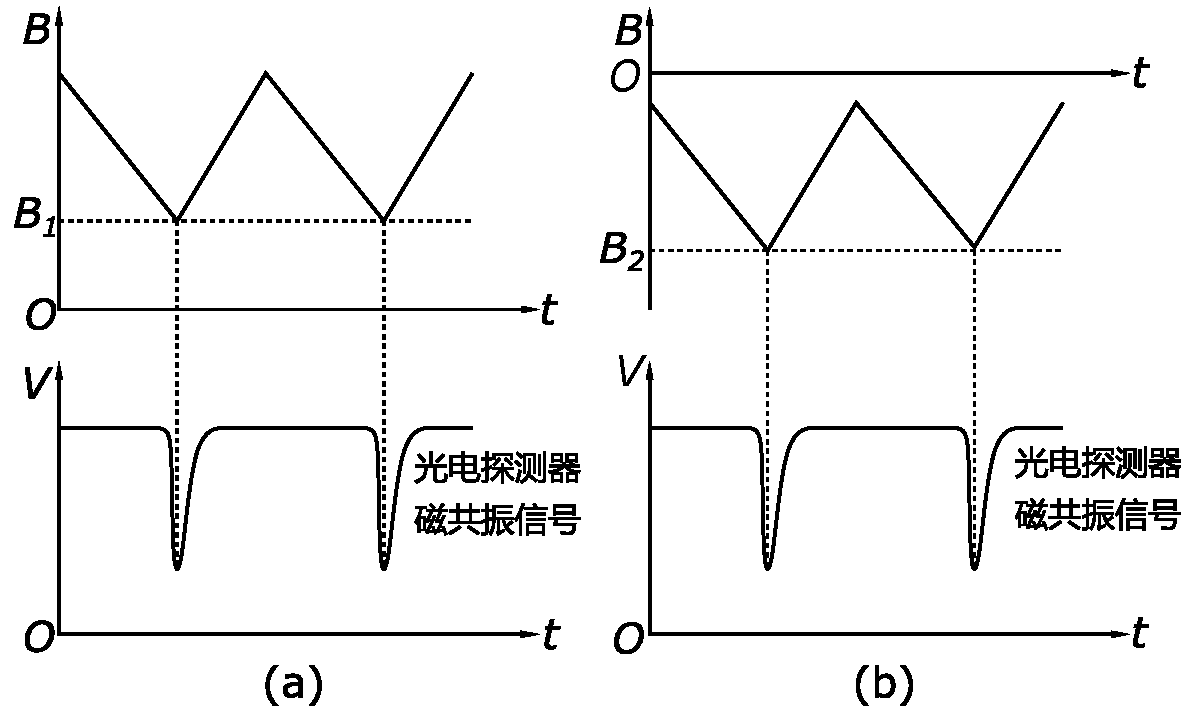
\includegraphics[width=0.8\textwidth]{fig/fig5.pdf}
\caption{测量$g_F$因子原理图}\label{fig5}
\end{figure}
\item 实验第二步:改变水平场方向,仍用上述方法得到频率$\nu_2$,对应的总的水平场为$|B_2| = -B_2 = B_{\text{水平}} - B_{\text{地水平}} - B_{\text{扫}}$,如图(\ref{fig5}-b)所示。将$\nu_1$,$|B_1|$和$\nu_2$,$|B_2|$分别代入(\ref{eq4})式,然后两式相加,得到$|g_F| = \frac{h\nu}{\mu_BB_{\text{水平}}}$。其中$B_{\text{水平}}$对应的频率为$\nu = \frac{\nu_1 + \nu_2}{2}$,这样就消除了地磁场水平分量和扫场的影响。从(\ref{eq4})式还可看出,当水平方向总磁场$|B|$不变时,磁共振频率$\nu$跟$g_F$成正比。由于存在基态$5^2\text{S}_{\frac{1}{2}}$,$^{87}$Rb与$^{85}$Rb的$|g_F|$值不同,所以它们的共振频率也不同,$^{87}$Rb的$|g_F|$值大,它的共振频率也高。因此在实验第一步和第二步中,都会测出两个高低不同的共振频率,分别属于$^{87}$Rb和$^{85}$Rb。本实验就是用的这种固定水平磁场而调节射频频率的方法,称为调频法。

在基态$5^2\text{S}_{\frac{1}{2}}$,$J=\frac{1}{2}$,最大的$F=I+J=I+\frac{1}{2}$,代入(\ref{eq3})式将其化简为
\begin{equation}
g_F = \frac{g_J}{2I+1}\label{eq5}
\end{equation}
从而
\begin{equation}
I = \frac{g_J - g_F}{2g_F}\label{eq6}
\end{equation}
已知基态的$g_J=2$和实验测定的正值$g_F$,代入(\ref{eq6})式,就能定出$^{87}$Rb和$^{85}$Rb的核自旋量子数$I$。将$g_F$和$I$的实验测定值与理论值相比较,计算其误差。

光磁共振实验还可以采用固定射频频率而调节水平磁场的方法(称为调场法)进行。从(\ref{eq4})式可以看出,当射频频率$\nu$不变时,水平方向总磁场$|B|$与$|g_F|$成反比,因此$|B|$大的为$^{85}$Rb的共振信号,$|B|$小的为$^{87}$Rb的共振信号。还要注意的是,因为三角波扫场的波峰和波谷处的磁感应强度不同,故对每一同位素将分别在波峰和波谷处观察到不同频率的磁共振信号。
\end{enumerate}
\subsection{测定地磁场的水平分量$B_{\text{地水平}}$和倾角$\theta$}
本实验装置实际上是一台铷原子磁强计,可以利用射频磁共振关系(\ref{eq4})式,由实验上测定的$\nu$和$|g_F|$来确定水平方向总磁场$|B|$。跟测$g_F$得分方法类似,先使扫场$\bm{B}_{\text{扫}}$和水平磁场$\bm{B}_{\text{水平}}$与地磁场水平分量$\bm{B}_{\text{地水平}}$方向相同,测得射频共振频率$\nu_1$,对应有$h\nu_1 = |g_F|\mu_BB_1 = |g_F|\mu_B(B_{\text{水平}} + B_{\text{扫}} + B_{\text{地水平}})$。为了测$B_{\text{地水平}}$,要消除$\bm{B}_{\text{水平}}$和$\bm{B}_{\text{扫}}$的影响,于是同时改变水平磁场$\bm{B}_{\text{水平}}$和扫场$\bm{B}_{\text{扫}}$的方向,使之跟地磁场水平分量$\bm{B}_{\text{地水平}}$的方向相反,测得射频共振频率$\nu_3$,有$h\nu_3 = |g_F|\mu_BB_3 = |g_F|\mu_B(B_{\text{水平}} + B_{\text{扫}} - B_{\text{地水平}})$,两式相减,得到$B_{\text{地水平}} = \frac{h\nu}{\mu_B|g_F|}$,其中跟$B_{\text{地水平}}$相对应的频率$\nu = \frac{v\nu_1 - \nu_3}{2}$,而$|g_F|$已在前面测得,这样便消除了扫场和水平场的影响,从而得到地磁场的大小和方向:
\begin{eqnarray}
B_{\text{地}} &=& \sqrt{B^2_{\text{地水平}} + B^2_{\text{地垂直}}}\label{eq7}\\
\tan\theta &=& \frac{B_{\text{地垂直}}}{B_{\text{地水平}}}\label{eq8}
\end{eqnarray}
其中$\theta$为地磁场$\bm{B}_{\text{地}}$的倾角。

\section{实验数据}

\section{误差分析}

\section{思考题}
\subsection{$^{87}$Rb的基态$F=1$与$F=2$的塞曼子能级排列相反,$^{85}$Rb的基态$F=2$与$F=3$的塞曼子能及排列也相反,是何原因?}
\subsection{测量$g_F$值时,将水平换向得到的频率为$\nu = \frac{\nu_1+\nu_2}{2}$,为什么不是$\nu = \frac{\nu_1-\nu_2}{2}$?必须满足的条件是什么?测地磁场水平分量时,得到的频率为什么是$\nu = \frac{\nu_1-\nu_3}{2}$?相应的条件又是什么?}
\subsection{为什么实验要在抵消地磁场垂直分量的状态下进行?}
\subsection{扫场在实验中的作用是什么?}
\subsection{为什么射频磁场必须在竖直方向,跟产生塞曼子能级的稳定弱磁场相垂直?}
\subsection{如果射频信号频率是相邻塞曼子能级间隔的两倍,能否产生由$m_F = +2$到$m_F = 0$的磁共振?为什么?}


\section*{附录}

\begin{appendix}
\section{亥姆霍兹线圈轴中心处磁感应强度B的计算公式}
\begin{equation}
B = \frac{16\pi}{5^{\frac{3}{2}}}\frac{NU}{rR}\times 10^{-7}\text{T}\label{eq9}
\end{equation}
式中:N为线圈每边匝数;R为线圈线绕电阻($\Omega$);r为线圈有效半径(m);U为线圈上加的直流电压(V)。其中各线圈的N,r,R等参数实验室已给出,U由数字电压表读出。
\end{appendix}

\nocite{jiaocai}
\bibliography{ref}
\end{document}